\documentclass{article}

% Language setting
% Replace `english' with e.g. `spanish' to change the document language
\usepackage[english]{babel}

% Set page size and margins
% Replace `letterpaper' with `a4paper' for UK/EU standard size
\usepackage[letterpaper,top=2cm,bottom=2cm,left=3cm,right=3cm,marginparwidth=1.75cm]{geometry}

% Useful packages
\usepackage{amsmath}
\usepackage{amsthm}
\usepackage{listings}
\lstset{language     = Matlab,
        numbers      = left,
        numbersep    = 5pt,
        numberstyle  = \small\color{red},
        keywordstyle = \color{cyan},
        rulecolor    = \color{black},
        commentstyle = \color{green},
        frame        = single,
        keepspaces   = true,
        tabsize      = 4,
        }
\usepackage{graphicx}
\usepackage{subfigure}
\usepackage{setspace}
\usepackage{float}
% \usepackage[ruled]{algorithm2e}
\usepackage{booktabs}

\usepackage{graphicx} % Allows including images
\usepackage{animate}
% \usepackage{algorithm}
% \usepackage{algorithmic}
\usepackage[ruled,linesnumbered]{algorithm2e}

\usepackage[english]{babel}
\newtheorem{theorem}{Theorem}
\newtheorem{definition}{Definition}
\newtheorem{lemma}{Lemma}[section]

\usepackage[colorlinks=true, allcolors=blue]{hyperref}

%%%%%%%%% TITLE - PLEASE UPDATE
\title{Realtime And Editable Mandelbrot Set on GPU}

\author{Qihe Chen\\
% ShanghaiTech University, China\\
% Shanghai Road Zhongke\\
{\tt\small chenqh@shanghaitech.edu.cn}
% For a paper whose authors are all at the same institution,
% omit the following lines up until the closing ``}''.
% Additional authors and addresses can be added with ``\and'',
% just like the second author.
% To save space, use either the email address or home page, not both
\and
Haiyu Song\\
% ShanghaiTech University, China\\
% Shanghai Road Zhongke\\
{\tt\small songhy@shanghaitech.edu.cn}
}

\begin{document}
\maketitle

\begin{abstract}
    In this final programming project, we implement Mandelbrot Set on GPU with editable features and realtime rendering high performance. Since the Mandelbrot set is generated by iteration, it is almost impossible to make the parallelization for single pixel color calculation. Therefore, we focus on the parallelization of warps of pixels instead of single pixel. To the rendering part, we implement two techniques on GPU, i.e. phong lighting and stripe average coloring. To the experimental part, we implement two kinds of Mandelbrot Set, i.e. basic algorithm and escaped time based algorithm. To the evaluation part, we compare our method with serial method on basic algorithm.
\end{abstract}

\section{Introduction}
    We implement the Mandelbrot Set on GPU and build a rendering framework by OpenGL and Dear Imgui.
    \subsection{Compile \& Build}
        We recommend to compile the project on Windows 10 operation system. For compiling successfully, g++ should support at least C++ 17 standard and nvcc should support at least C++ 17 also.
        
        We recommend we to build the project by CMake with version at least 3.21.

\begin{lstlisting}[language=bash]
mkdir build
cd ./build
cmake ..
cmake --build . --config Release
./Release/main.exe
\end{lstlisting}

     It should compile successfully and automatically run the executable file.

    \subsection{Benchmark Configures}
        \begin{table}[h]
        \centering
        \begin{tabular}{@{}c|c@{}}
        \toprule
        Config   & Value   \\ \midrule
        CPU      & Intel(R) Core(TM) i9-10900x CPU @ 3.70GHz \\
        GPU     &  NVIDIA GeForce RTX 3090  \\ 
        Memory   & 64 GB DDR4 3200 MHz 2 of 8 slots   \\
        GPU Memory & 24576 MB GDDR6X (Micron)  \\
        OS       & Windows 10 21H2 19044.2251  \\
        Compiler &  MSVC 19.33.31630.0, nvcc V11.8.89   \\
        Optimize & MSVC: /O2, nvcc: -O3  \\ 
        CUDA Cores   & 10496 \\
        Bandwidth & 936.2GB/s \\
        Driver Version & 31.0.15.2206 (NVIDIA 522.06) DCH / Win 10 64\\
        \bottomrule
        \end{tabular}
        \end{table}

    \subsection{Mandelbrot Set}
        The Mandelbrot set is the set of complex numbers $c$ for which the function 
        $f_{c}(z)=z^{2}+c$ does not diverge to infinity when iterated from $z=0$, 
        i.e., for which the sequence $f_{c}(0)$, $f_{c}(f_{c}(0))$, etc., remains 
        bounded in absolute value.\cite{wiki:Mandelbrotset}
        \begin{figure}[H]
        	\centering
        	
\includegraphics[width=0.6\linewidth]{mandelbrotset.jpg}
        	\caption{MandelbrotSet}
        \end{figure}
        For a complex $z$, given parameter complex $c$, we define $f$ function below:
            \begin{equation}
                f_c(z)=z^2+c
            \end{equation}
        If the orbit of the critical point $z=0$ under iteration of quadratic marginparwidth
            \begin{equation}
                z_{n+1}=z_n^2+c
            \end{equation}
        remains bounded. We say that the complex number $c$ is a member of the Mandelbrot Set, when 
        starting with $z_0=0$ and applying the iteration repeatedly, the absolute value of $z_n$ remains 
        bounded for all $n>0$.

    \subsection{Speed up}
        We evaluate the performance of our GPU-version Mandelbrot Set by comparing the running time to render a $800\times 600$ frame with CPU-version under different max iterations. For stability, we continue to render frames until the average fps converging. And the CPU-version is accelerated by OpenMP.

    \begin{table}[H]
    \centering
    \begin{tabular}{ccccc|c}
    \hline
    maxiter & \begin{tabular}[c]{@{}c@{}}CPU\\ ms/frame\end{tabular} & \begin{tabular}[c]{@{}c@{}}GPU\\ ms/frame\end{tabular} & \begin{tabular}[c]{@{}c@{}}CPU\\ fps\end{tabular} & \begin{tabular}[c]{@{}c@{}}GPU\\ fps\end{tabular} & speed up \\ \hline
    100     & 113.081                                                & 7.225                                                  & 8.8                                               & 138.4                                             & 15.651   \\
    200     & 217.070                                                & 10.148                                                 & 4.6                                               & 98.5                                              & 21.390   \\
    300     & 307.077                                                & 14.200                                                 & 3.3                                               & 70.5                                              & 21.625   \\
    500     & 495.950                                                & 22.303                                                 & 2.0                                               & 44.9                                              & 22.237   \\
    1000     & 942.430                                                & 42.444                                                 & 1.1                                               & 23.6                                              & 22.204   \\
    2000    & 1876.767                                               & 83.336                                                 & 0.5                                               & 12.0                                              & 22.520   \\ \hline
    average &                                                        &                                                        &                                                   &                                                   & 20.92    \\ \hline
    \end{tabular}
    \end{table}
        
        
\section{Preliminary}
    \subsection{Mandelbrot Set}
        \subsubsection{Definition. } The Mandelbrot set is generated by iteration, which means to repeat a process over and over again. In mathematics, this process is most often the application of a mathematical function. For the Mandelbrot set, the functions involved are some of the simplest imaginable: they all are what is called \textit{quadratic polynomials} and have the form $z_{t+1}=z_t^2+c$, where \textit{c} is a constant number.

        \subsubsection{Mathematics. } From the mathematical view, the Mandelbrot set is a mathematical set of points that is defined in the complex plane. The set is define using an iterative process that involves performing a simple mathematical operation on a complex number repeatedly. This operation is defined by the equation:

        \begin{equation}
            \label{equ:iter}
            z=z^2+c
        \end{equation}

        where $z$ and $c$ are complex numbers. The mandelbrot set is the set of all complex numbers $c$ for which the above equation does not diverag, that is , the absolute value of $z$ remains less than $2$ for all iterations. The equation is repeated a large number of times to determine whether a given number is in the set or not.
        
        \begin{lemma}
	   A point $c$ belongs to the Mandelbrotset if and only if $|z_n| \leq 2$ for all $n \geq 0$.
        \end{lemma}
        
        \begin{proof}
        	if $|z_j|>2$, we can write $|z_j|$ as $|z_j|=2+\varepsilon$ for $\varepsilon \in \mathcal{R}^+$\\
        	$$\begin{aligned}
        		|z_j^2|&=|z_j^2+c-c|\\
        			&\geq|z_j^2+c|+|c|\\
        		|z_{j+1}|&=|z_j^2+c|\\
        		&\geq |z_j|^2-|c|\\
        		&\geq |z_j|(|z_j|-1)\\
        		&\geq |z_j|(1+\varepsilon)
        	\end{aligned}$$
        	So, after k iterations, we have $$|z_{j+k}^2+c|\geq |z_j|(1+\varepsilon)^k$$
        	which escapes to infinity.\\
        	Since $c=z_{1}$, it follows that $|c|\leq 2$, establishing that $c$ will always be in 
        	the closed disk of radius 2 around the origin.
        \end{proof}
        
        \subsubsection{Background}
            
        The Mandelbrot set is interesting because it exhibits a complex and intricate structure when plotted, with a seemingly infinite level of detail. It has become famous for its aesthetic appeal and has been featured in many works of art, music, and literature. It is also studied in mathematics for its connection to the field of fractals, which are geometric shapes that are self-similar and exhibit a repeating pattern at different scales.

    \subsection{Phong Lighting}
        Phong lighting is a type of 3D computer graphics shading techique, which is extended to 2D Mandelbrot Set shading in this project. In the Phong lighting model, the intensity of the reflected light at any point on a surface is a combination of three components: ambient light, diffuse relfection, and specular reflection.

        \begin{itemize}
            \item Ambient light is the base level of light that is present in a scene, and it is evenly distributed over all surfaces.
            \item Diffuse reflection is the light that is scattered evenly in all directions after it his a rough surface.
            \item Specular reflectuion is the light that is reflected in a specific direction, producing a highlight or a shiny spot on a surface.
        \end{itemize}

        The Phong lighting model is typically implemented in computer graphcis using the following equation:

        \begin{equation}
            \label{equ:phong}
            L=I_aK_a+I_dK_d\max(0,n\cdot I) + I_sK_s\max(0, n\cdot h)^p
        \end{equation}

    \subsection{Stripe Average Coloring}
        Stripe average coloring is a post-processing technique for creating color schemes for fractals. The technique involves creating color bands or "stripes" of uniform color and then blending or averaging the colors of adjacent stripes to create a smooth gradient effect. In this project, it can be used to create colorful and visually appealing images of fractals.
    
\section{Method}

    \subsection{Basic Algorithm}
        \begin{algorithm}[H]  %其中这里面不能有H不然会报错,不过不影响结果
        	\caption{Escape Algorithm}%算法名字
        	\LinesNumbered %要求显示行号
        	\KwIn{complex c, maxiteration}%输入参数
        	\KwOut{iteration count}%输出
        	z $\leftarrow$ 0\\
        	count $\leftarrow$ 0\\
        	\For{i=1 \textup{to maxiteration and abs(z)} $\textless$ 2}{
        		z $\leftarrow$ $z^2$+c\\
        		count $\leftarrow$ count+1
        	}
        	return count
        \end{algorithm}
    
    \subsection{Visualization}
        In this project, we use OpenGL to help us rendering the image realtime and use third library "imgui" to 
        better GUI to control the input parameter and selcet the drawing mode.\\

        \subsubsection{Coloring}
            We use colortable to color the pixel according to their iteration count.\\
            We produce the colortable using sin function and convert from [0,1] to [0,255] later.
            \begin{algorithm}[]
            	\caption{ColorTable Algorithm}
            	\LinesNumbered %要求显示行号
            	\KwIn{theta, colorsize}%输入参数
            	\KwOut{colortable}%输出
                dx $\leftarrow$ 1 / colorsize\\
            	colors $\leftarrow$ empty vector\\
                \For{i=0 \textup{to colorsize}}
                {
                    color $\leftarrow$ (vec3(dx * i) + theta) * 2 * PI\\
                    color $\leftarrow$ 0.5+0.5*sin(y)\\
                    colors[i] $\leftarrow$ color\\
                }
                return colors
            \end{algorithm}

        \subsubsection{Color smooth}
            We use smoother function to smooth number of iteration in the Mandelbrot set for given c.\\
            In this funciton, we combine the frequency parameter and memory parameter to control the stripe average Coloring.\\
            In particular, we use "Jussi Harkonen On Smooth Fractal Coloring Techniques" to stripe average coloring and use 
            "Smoothing + linear" to interpolate.\\
            \begin{algorithm}[]
            	\caption{Smoother Algorithm}
            	\LinesNumbered %要求显示行号
            	\KwIn{complex c, stripe\_s,stripe\_sig}%输入参数
            	\KwOut{niter, stripe\_a, dem,normal}%输出
            	z $\leftarrow$ 0\\
                dz $\leftarrow$ 1\\
            	esc\_radius $\leftarrow$ 1e5\\
            	stripe\_a $\leftarrow$ 0\\
            	\For{n=0 to maxiter}{
            		dz $\leftarrow$ (2*z*dz)+1\\
            		z $\leftarrow$ z*z+c\\
            		stripe\_tt $\leftarrow$ (sin(stripe\_s*atan2(z.imag, z.real)) + 1) / 2\\
            		\If{abs(z) $\textgreater$ esc\_radius}{
            			modz $\leftarrow$ abs(z)\\
            			log\_ratio $\leftarrow$ log(modz) / log(esc\_radius)\\
            			smooth\_i $\leftarrow$  1 - log(log\_ratio) / log(2)\\
            			stripe\_a $\leftarrow$ (stripe\_a * (1 + smooth\_i * (stripe\_sig-1)) + stripe\_t * smooth\_i * (1 - stripe\_sig))\\
                        stripe\_a $\leftarrow$ stripe\_a / (1 - pow(stripe\_sig, n) * (1 + smooth\_i * (stripe\_sig-1)))\\
            			normal  $\leftarrow$ z/dz\\
            			dem $\leftarrow$ modz * log(modz) / abs(dz) / 2\\
            			return (n+smooth\_i, stripe\_a, dem, normal)\\
            		}
            		stripe\_a $\leftarrow$ stripe\_a * stripe\_sig + stripe\_tt * (1 - stripe\_sig)\\
            	}
            	return (0,0,0,\{0, 0\})
            \end{algorithm}
        
        \subsubsection{Phong lighting}
            We use Lambert normal shading for better visualization.\\
            The color of a pixel is 
            $$  \textup{result = ambient + diffuse + specular}$$
            \begin{algorithm}[H]  %其中这里面不能有H不然会报错,不过不影响结果
            	\caption{Phong lighting Algorithm}%算法名字
            	\LinesNumbered %要求显示行号
            	\KwIn{complex normal, light}%输入参数
            	\KwOut{brightness}%输出
            	normal $\leftarrow$ normalize\\
            	diff $\leftarrow$ normal.real*cos($\phi$)*cos($\theta$) +
            	normal.imag*sin($\phi$)*cos($\theta$) +sin($\theta$)\\
            	diff $\leftarrow$ diff/(1+sin($\theta$))\\
            	thetahalf $\leftarrow$ (pi/2 + $\theta$)/2\\
                spec $\leftarrow$ normal.real*cos($\phi$)*sin(thetahalf) +
                         normal.imag*sin($\phi$)*sin(thetahalf) +cos(thetahalf)\\
                spec $\leftarrow$ spec/(1+cos(thetahalf))\\
                spec $\leftarrow$ spec ** shininess \\
                bright $\leftarrow$ k\_ambient + k\_diffuse*diff + k\_specular*spec\\
                bright $\leftarrow$ bright * opacity + (1-opacity)/2 \\
                return bright
            \end{algorithm}

    \subsection{Optimization}
        \subsubsection{Cuda parallel}
            Since calculating for each pixel are independent and the workload are nearly balanced. Thus, we 
            can use Cuda to help us generate the image quickly.\\
            Naturally, we use $*data$ to store the whole pixel with size $width*height$. And we equally divide the 
            data calculation work for each block.\\
    
        \subsubsection{Memory access and allocation}
            Since there are many data pass from device to host when we draw pictures, we don't need to malloc 
            cudamemory each time when we call Cuda kernel.\\
            Instead, we just assign memory for host and device respectively once, and each time we call cuda kernel, 
            we just pass the pointer to cuda. When we need to feed back the data from device, we simply transfer the 
            the data from device to host with the help of \textless thrust/host\_vector.h\textgreater and \textless thrust/device\_vector.h\textgreater.\\
            
\section{Experiment}
    \begin{figure}[H]
        \centering
        \subfigure[pic1.]{
        \begin{minipage}[t]{0.5\linewidth}
        \centering
        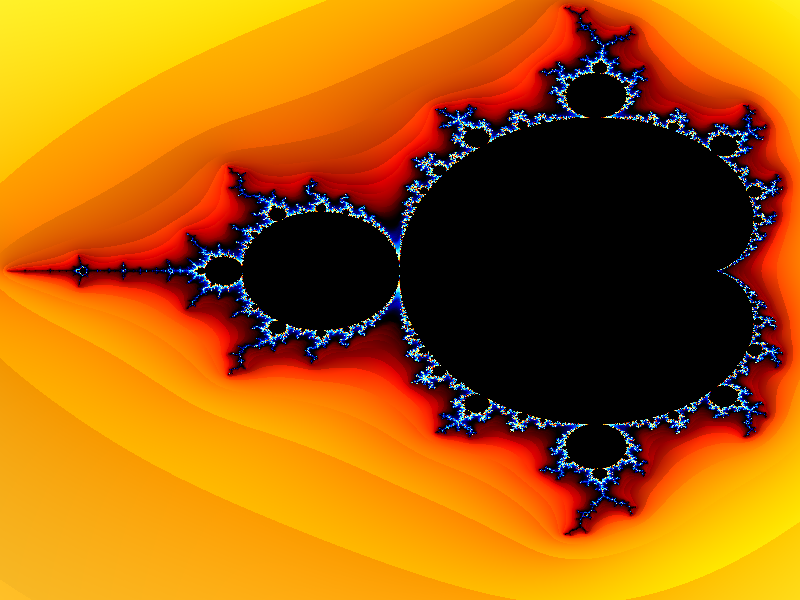
\includegraphics[width=\linewidth]{MandelbrotSet1.png}
        %\caption{fig1}
        \end{minipage}%
        }%
        \subfigure[pic2.]{
        \begin{minipage}[t]{0.5\linewidth}
        \centering
        
\includegraphics[width=\linewidth]{MandelbrotSet2.png}
        %\caption{fig2}
        \end{minipage}%
        }%
        \quad             %这个回车键很重要 \quad也可以
        \subfigure[pic3.]{
        \begin{minipage}[t]{0.5\linewidth}
        \centering
        
\includegraphics[width=\linewidth]{MandelbrotSet3.png}
        %\caption{fig2}
        \end{minipage}
        }%
        \subfigure[pic4.]{
        \begin{minipage}[t]{0.5\linewidth}
        \centering
        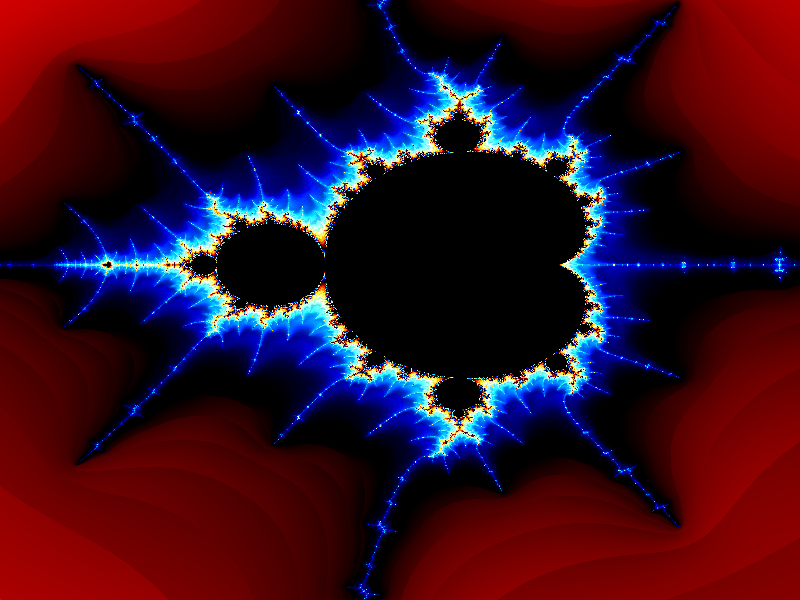
\includegraphics[width=\linewidth]{MandelbrotSet4.png}
        %\caption{fig2}
        \end{minipage}
        
        }%
        
        \centering
        \caption{ pics}
        \end{figure}
        
        \begin{figure}[H]
        \centering
        
        \subfigure[pic1.]{
        \begin{minipage}[t]{0.5\linewidth}
        \centering
        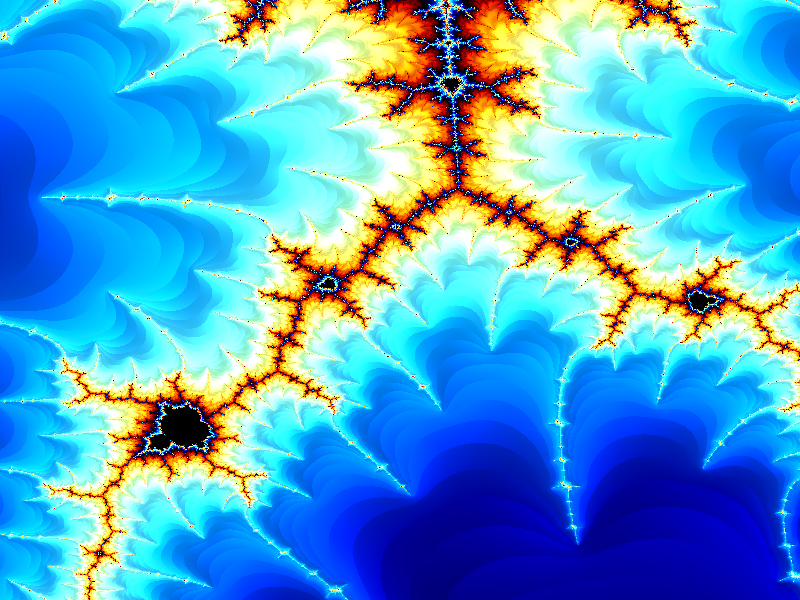
\includegraphics[width=\linewidth]{MandelbrotSet5.png}
        %\caption{fig1}
        \end{minipage}%
        }%
        \subfigure[pic2.]{
        \begin{minipage}[t]{0.5\linewidth}
        \centering
        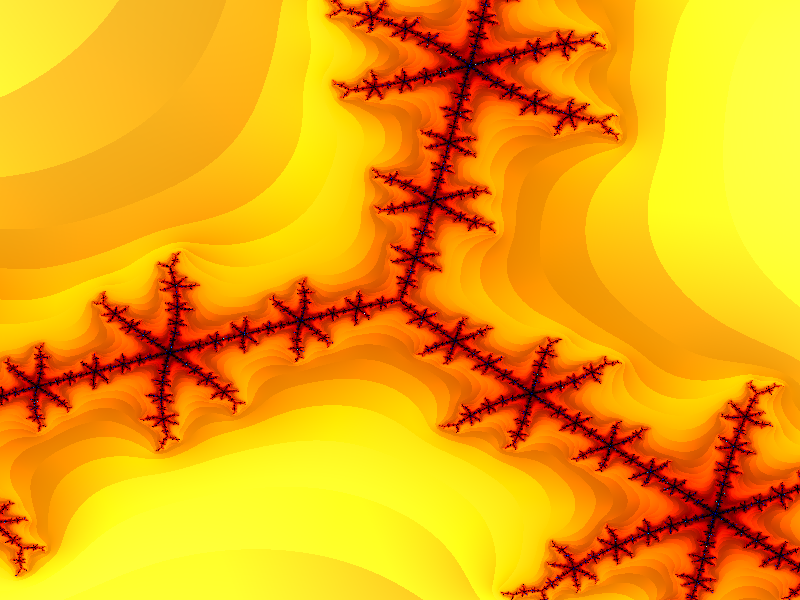
\includegraphics[width=\linewidth]{MandelbrotSet6.png}
        %\caption{fig2}
        \end{minipage}%
        }%
        \quad             %这个回车键很重要 \quad也可以
        \subfigure[pic3.]{
        \begin{minipage}[t]{0.5\linewidth}
        \centering
        
\includegraphics[width=\linewidth]{MandelbrotSet7.png}
        %\caption{fig2}
        \end{minipage}
        }%
        \subfigure[pic4.]{
        \begin{minipage}[t]{0.5\linewidth}
        \centering
        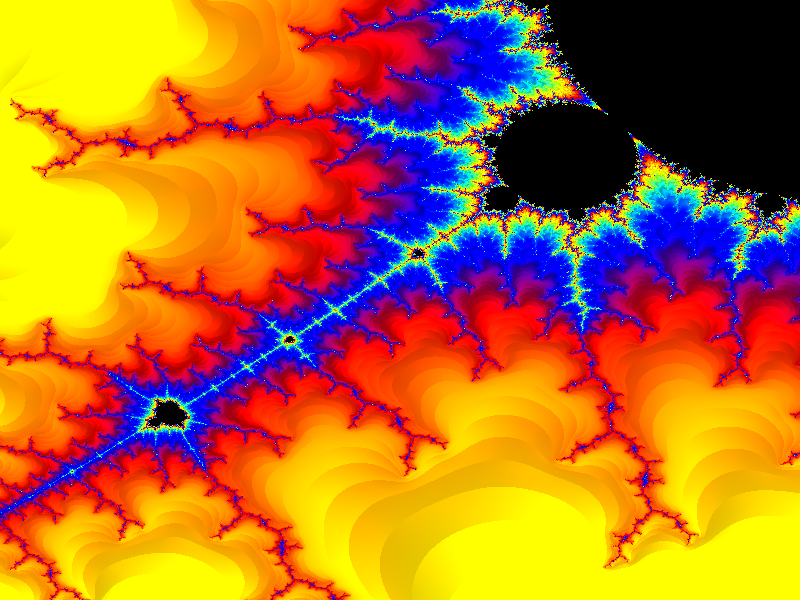
\includegraphics[width=\linewidth]{MandelbrotSet8.png}
        %\caption{fig2}
        \end{minipage}
        
        }%
        
        \centering
        \caption{ pics}
    \end{figure}



\begin{center}
\animategraphics[autoplay,
					loop,
					controls,
					width=.7\textwidth]{24}{./gif2/set-}{0}{666}
\end{center}
\section{Conclusion}
    In this final programming project, we implement Mandelbrot Set on GPU with editable features and realtime rendering high performance. Since the Mandelbrot set is generated by iteration, it is almost impossible to make the parallelization for single pixel color calculation. Therefore, we focus on the parallelization of warps of pixels instead of single pixel. To the rendering part, we implement two techniques on GPU, i.e. phong lighting and stripe average coloring. To the experimental part, we implement two kinds of Mandelbrot Set, i.e. basic algorithm and escaped time based algorithm. To the evaluation part, we compare our method with serial method on basic algorithm. Finally, we achieve 20x times speed up than traditional openmp serial algorithm.



\bibliographystyle{alpha}
\bibliography{ref}

\end{document}
